\chapter{知识图谱概述}\label{sec:Background}
\section{什么是知识图谱}
当我们在百度“瓦特”的时候,百度会返回发明家瓦特的百度百科等页面(如图\ref{fig:baiduWatt})。为什么会这样?
因为百度为所有网页建立了从关键词到网页的倒排索引。基于倒排索引,百度首先找到了包含“瓦特”的网页,然后百度基于PageRank算法对这些网页按照权威程度进行排序,最后最权威的网页(如瓦特的百度百科页面)被排在前面返回给我们。

换言之,瓦特的百度百科页面被返回的原因并不在于计算机知道那个网页描述了瓦特,而是在于这个网页包含了“瓦特”这两个字。

\begin{figure}
\begin{center}
   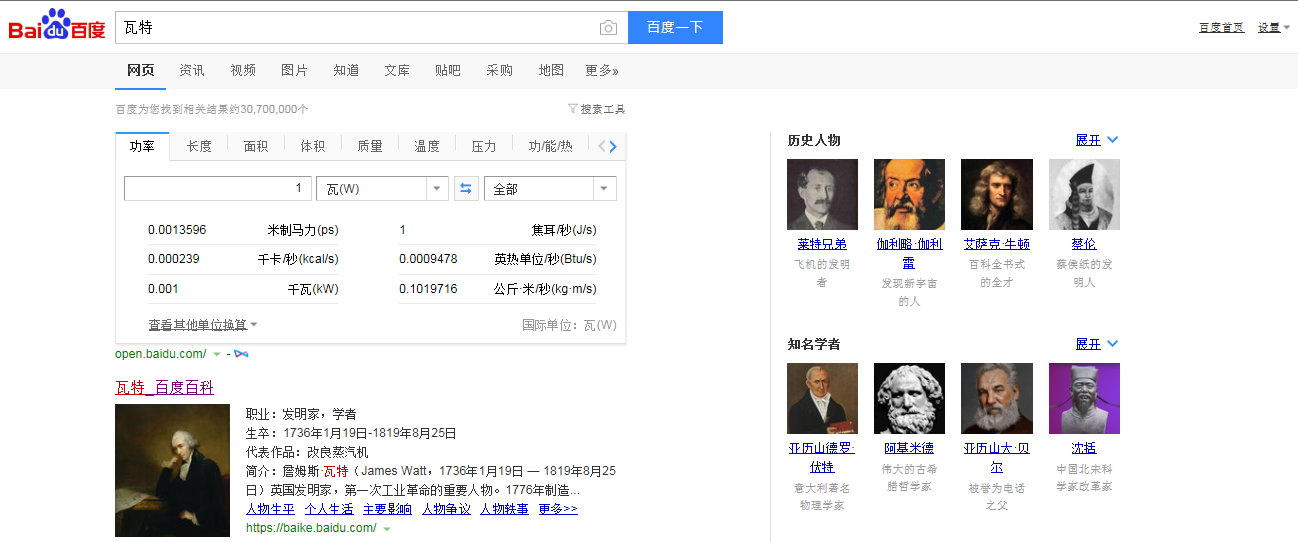
\includegraphics[width=12cm]{./figures/part1/baidu.png}
    \caption{百度“瓦特”结果页面}
   \label{fig:baiduWatt}
\end{center}
\end{figure}


上面这些基于文本字符串的技术,在这些年的互联网发展中取得不错的效果,已经成为了目前互联网上进行自然语言理解的基础。谷歌、百度等一系列搜索引擎基于这些技术成长为了行业巨头。


但是随着时代发展,这些技术的局限性也日益明显。因为基于文本字符串的技术本质上并没有理解我们的语义,所以它无法处理复杂的带语义的查询。比如当我们查询“瓦特在哪工作过?”的时候,百度会给我们返回一系列百度知道、百度贴吧的问答(如图\ref{fig:baidufatherinlaw}),而无法直接返回“格拉斯哥大学”的相关页面。这本质上就是因为搜索引擎只是根据网页中的文本内容来得到结果,而不是真正理解我们的世界。

\begin{example}\textbf{(背景知识)}

\emph{詹姆斯·瓦特}(James Watt,1736年1月19日 — 1819年8月25日)英国发明家,出生于苏格兰的港口小镇格林诺克(Greenock),第一次工业革命的重要人物。他于1776年制造出第一台有实用价值的蒸汽机,进而开辟了人类利用能源新时代,使人类进入“蒸汽时代”。后人为了纪念这位伟大的发明家,把功率的单位定为“瓦特”(简称“瓦”,符号W)。\footnote{https://baike.baidu.com/item/詹姆斯·瓦特}

\emph{格拉斯哥大学}(University of Glasgow),英国老牌名校,位于英国苏格兰格拉斯哥市,始建于1451年,是全球最为古老的十所大学之一,英语世界国家第四古老大学。
作为一所英国综合性古典大学,格拉斯哥大学与人类文明的发展紧密相联。经济学之父亚当·斯密(Adam Smith)、工业革命之父詹姆斯·瓦特等大批杰出校友均为社会的发展进步做出了举世瞩目的贡献。\footnote{https://baike.baidu.com/item/格拉斯哥大学}

1757年,格拉斯哥大学的教授提供给瓦特一个机会,让他在大学里开设了一间小修理店。其中的一位教授,物理学家与化学家约瑟夫·布莱克(Joseph Black)更是成了瓦特的朋友与导师。瓦特的小店开业5年后,在朋友的引导下,瓦特开始了对蒸汽机的实验。经过近20年的研发,1774年瓦特将自己设计的蒸汽机投入生产,并于1776年成功制造了第一批新型蒸汽机并应用于实际生产。
\end{example}

\begin{figure}
\begin{center}
   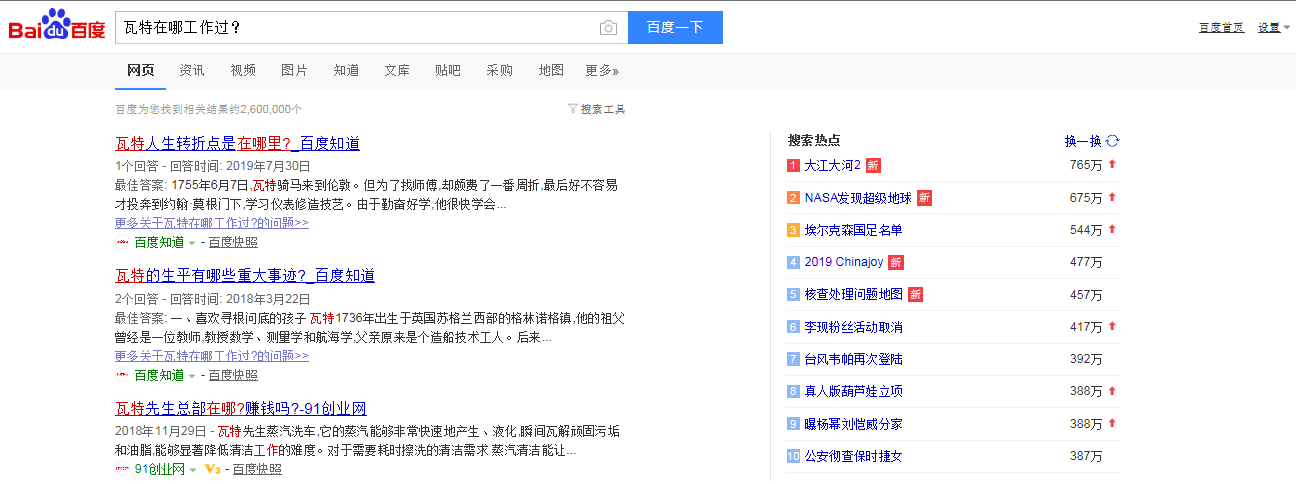
\includegraphics[width=12cm]{./figures/part1/baidufatherinlaw.png}
    \caption{百度“瓦特在哪工作过?”结果页面}
   \label{fig:baidufatherinlaw}
\end{center}
\end{figure}

为了让计算机更加智能,让计算机理解我们的世界,于是我们需要计算机理解这个世界的知识。


知识是结构化的经验、价值、相关信息和专家洞察力的融合,并为新经验的评估、整合与资讯等提供架构\cite{url:KnowledgeDef}。20世纪90 年代以来,万维网已成为人们获取知识的主要的手段\cite{article:Internet}。为了在万维网上的获取知识,人们通常通过向搜索引擎提交关键词的方式从万维网上检索出通过网页文本、图片、视频等形式所呈现出的信息,并从这些信息里面提取所需知识。


近些年来,知识图谱(Knowledge Graph)逐渐兴起并成为互联网上表示知识并利用知识的重要发展方向。知识图谱是由谷歌公司于2012年5月16日正式发布出来,用来增强谷歌搜索引擎的能力\cite{url:KnowledgeGraphDef}。
在知识图谱中,人们将越来越多的知识按照图的形式结构化地组织起来。这些图结构化、易操作、易利用、全面有组织的知识集群就是知识图谱。知识图谱经常是采用某种知识表示模型在计算机存储器中存储、组织、管理和使用的互相联系的知识片集合。

构建知识图谱的本质,就是让机器具备认知能力,理解这个世界。

\section{知识图谱由来与发展}
知识图谱源于专家系统与知识工程,是人工智能学科符号主义分支的最新研究成果。
1956年夏,麦卡锡、明斯基等科学家在美国达特茅斯学院开会研讨“如何用机器模拟人的智能”,首次提出“人工智能(Artificial Intelligence,简称AI)”这一概念,标志着人工智能学科的诞生。而这些科学家都是符号主义者。正是这些符号主义者,早在1956年首先采用“人工智能”这个术语。直到2012年,谷歌提出了“知识图谱”概念,将符号主义这一分支又推向了新的高度。

知识图谱这个概念虽然是2012年之后才为大家所知的,但是这个技术继承了符号主义几十年的积累。从1956年人工智能学科符号主义分支形成以来,符号主义分支走过了一条启发式算法——专家系统——知识工程的发展道路。

在六十年代、七十年代的时候,知识工程这个领域往前发展,不断的产生出新的逻辑语言和新的实用方法,像描述逻辑是七十年代就兴起了的。在六十年代时就有一个叫语义网络。注意,不是“语义网”而是“语义网络 ”,那个时候的语义网络跟现在的知识图谱非常像。所以这个是不断循环的,如果我们把六十年的学科发展抽象来看,实际上就是一个从简单到复杂、再从复杂回归简单的过程。

从最终得到的结果来看,好像我们现在得到的知识图谱跟六十年代就已经有的语义网络非常像,但这种像只是表面上的。因为在发展过程中,我们构造了一个庞大的工业体系,以及如何从各种各样的文档、各种各样的数据里集中编辑、生成知识图谱的一整套工业链。所以一个技术不能只看它的定义,而是要看它相关所有实践过程中工业体系的总和。今天知识图谱的技术无论从深度还是广度上,都远远超越六十年代的语义网络技术。

八十年代、九十年代、到两千年,这中间还有非常多中间技术,我们从中选些重要的事情说一下。

这张图是对前面那张图的抽象,我们选其中发展过程中最重要的节点。六十年代有一种东西叫 “ 语义网络 ”,语义网络在七十年代、八十年代时演化成了描述逻辑。为什么会有这种变化?因为语义网络本身只是一种表征,并不具备推理能力。语义网络 + 推理变成了新的逻辑系统,叫 “ 描述逻辑 ”,描述逻辑到两千年前后跟 Web 技术结合在一起,形成了新的语言,比如 OIL 、DAML。

另外一个分支是 1995 年前后有了元数据,从元数据学科衍生出一个分支叫 RDF,后来 RDF 和 DAML 合并起来就变成了 OWL。下面还有一些更工程的内容,包括 schema.org、RDFa、JOSN-LD、GraphpDB,这都是最近 5、6 年兴起的新技术。这些技术的总和就构成了我们所称的 “ 知识图谱 ” 技术,但只是其中一部分。

给大家看一个语义网络,语义网络其实就是一个网络。这张图上有各种不同的概念,比如中间的 Mammal 是哺乳动物,猫(cat) 是一种哺乳动物,猫有毛;熊是哺乳动物,熊也有毛;鲸是一种哺乳动物,鲸在水里面生活;鱼也在水里面生活,也是一种动物;哺乳动物是一种脊椎动物,也是动物的一种。

所有这些节点和边的总和就构成了一个网络,每一条边上都有一些标志的,用术语来说就是 “ 有类型的边 ”,这种 “ 有类型的边 ” 连在一起的节点叫 “ 语义网络 ”,概念是非常简单的。

六十年代时自然语言处理和知识表现的大拿批评这种语义网络,说这个东西没办法用于推理,用术语来说是最后没有 “ semantics ”。

这里涉及很多关系,什么叫 semantics?有的学者认为 semantics 必须是有一套严格的语义定义,这通常是用模型论来定义,或者过程方法来定义。其实也有更浅的对语义的理解,万事万物之间的关系就是语义。比如我们打开字典,字典是用一些词定义另外一些词,这就是语义。

我们在这样的语义网络里,如何定义一个词的意义?其实我们是做不到的。比如在这个语义网络里,居于中间位置的词是“哺乳动物”,它到底是什么?我们很难让计算机理解什么是真正的哺乳动物,很难通过它的内涵含义来理解。对于计算机而言,它只能知道万事万物之间的联系,也许这对于机器自动处理来说就够了。所以语义网络尽管没有所谓的语义,我们还是把它称为语义网络的原因,因为语义就是关系。


到了八十年代时,描述逻辑就已经比较成熟了。描述逻辑是逻辑的一种,我在这里面列了一张表,这是描述逻辑和一阶逻辑 (FOL 逻辑)之间的对应。如果大家没有逻辑基础也不用害怕,因为这个图本质上是讲很基础的逻辑定义。

我们有了一个描述逻辑之后,就可以用计算机来做一些自动推理的工作。八十年代到九十年代,描述逻辑学者们一直都在寻找如何让计算机更好的进行逻辑推理,一些比较可判定的所谓计算机不会死机的那些问题的总和,这种语言称为 “ 描述逻辑 ”。


到九十年代时描述逻辑成为知识表现领域的一种非常显学、非常重要的分支,正好这时互联网兴起了。到了 1995 年前后开始了真正知识图谱化的第一步,开始把描述逻辑用互联网的语言来重新来表征,有人用 HTML,也有人用 XML。1999 年马里兰大学开始发布了第一个这样的语言,叫 “ SHOE ”。后来这个语言被美国的国防部高等研究所资助了一个项目叫 “ DAML ”,这就是第一个在美国这边把知识表现语言放在网上一种官方的努力。

与此同时,在欧洲也有一个非常相似的努力叫 “ OIL ”,大西洋两岸的同行们一看,大家做的事情非常相似,于是在 2001 年时 W3C 开始把两边的努力汇总在一起,出现了一个语言叫 “ DAML + OIL ”。到了 2004 年时 W3C 进一步协调大家的努力,合并了一个新的语言叫 “ OWL ”,2009 年发布了第二版,叫 “ OWL2 ”。

从九十年代到 2009 年这十几年期间,这个领域不断向上、向好积极发展,在那个时候我们曾经认为 OWL 是描述这个世界非常好的一种工具,因为它对于机器处理是非常友好的,所以我们就希望把它放到互联网上去,让更多人用到,但是这个设想后来并没有实现。


这里多说几句 OWL,因为我是 OWL 工作组的一员,所以知道一些早期的事情。OWL有两个工作组,最早的一个工作组是在 2000 - 2004 年之间,我赶上的是 2007 - 2010 年的第二个工作组,这个工作组的使命是把现有的 OWL 语言进一步完善,提供所谓更强的表达力,或者在机器处理上比如要进行语义数据的查询,我们应该用什么样的,什么可以用、什么不能用、什么能说、什么不能说、什么对机器是友好的,OWL 工作组就是做这个事情。

我们写了 10 来个文档,加在一起 600 多页纸,花了两年时间做这个事情。OWL 工作组除了大学里来的人,还有一些企业的成员,包括 IBM、Oracle、惠普等等,还有一些小的创业公司。

那个时候我们这个领域遇到了一些瓶颈的,就是 OWL 这个语言或者语义网整个领域,在 2000 年前后是大家非常寄予厚望的,就好像现在大家对于深度学习寄予厚望一样。但是往前走到 2006 年前后遇到了瓶颈,就是没有人真的去产生这样的数据,大多数日常场景用不到语义。于是这时候就产生了内部的路线斗争,叫 “ SEMANTIC Web or semantic WEB ”,就是到底我们是加强语义呢?还是加强互联网属性呢?有两组不同的人不断进行争执。

当然,还有很多其他的分歧,包括我们到底该怎么去定义什么叫 “ 简单 ”,大家没有一致的意见。所以我们最终生成的文档从学术角度来说是非常有价值,但是对于工业应用特别是 C 端的互联网应用没有达到预期。


前面这一段大体总结了知识图谱技术发展的前两个大的阶段历史,一个是从六十年代到九十年代,早期知识图谱的原型,包括语义网络等等,后面一系列的技术。

从 2001 - 2006 年或者 2007 年这段时间,是不断加强语义网所谓的语义的过程,就是从弱语义到强语义,从语义网络到描述逻辑,一直发展到 OWL,并行还有另外其他一些,比如基于框架逻辑还有另外一个语言叫 “ RIF ”。

这十几年时间都一直不断在加强语义表现的表达力,但最后证明这个做法是不太妥当的。


我们讲过,除了学术性非常强的描述逻辑 OWL 分支之外,知识图谱还有另外一个分支是来自于元数据框架的。这个工作最早是 Guha 在 Apple 做的,Guha 这个人是非常值得关注的,因为某种程度上他是 “ 知识图谱之父 ”,在 1995 年时他在 Apple 发明了一个语言叫 “ MCF ”,因为他那时候面临一些问题,就是怎么去表征多媒体的数据,特别是图像的数据,所以他就发明了一整套的元数据表征方法。

到了 1997 年时 Guha 跟Tim Bray 做了 RDF / XML。1999 年网景公司发明了 RSS 语言,这个东西现在新一代的朋友们不一定知道了,回到 10 年前时看新闻都是用 RSS 订阅的,其实 RSS 的第一个 R 就是 RDF。后来他们改了其他的名字,从本源上来讲,技术刚刚开始的时候这个技术是 RDF 的应用。1999 年 RDF 被 W3C 收编了,变成了国际标准。


RDF 和一开始提到描述逻辑方法是不一样的,因为描述逻辑方法是从实验室里来的,它想构造一个庞大的体系,构建一个完美的知识表现语言,然后再寻找它的落地。

而 RDF 从一开始就是一个从实践出发的、自底向上的一个语言。RDF 相对于 OWL 而言,是一个更加偏工程的、应用更多的语言,现在有很多人在用 RDF。我们日常生活中所遇到的绝大多数网站,现在都有某种类型的元数据,其中相当一部分就是用 RDF 不同的变种来实现的,所以 RDF 总的来说是一个比较成功的技术,因为它是来自于现实的技术。

从 2001 年这个领域正式形成,到 2006 年时语义网的技术堆栈已经变得非常复杂了。1999 年时有一个所谓的 “ 语义网蛋糕模型 ”,对语义网不同的技术做了罗列。2006 年时语义网技术已经复杂到没有人看得懂,没有办法用二维表达,必须用一个三维的图才能够把语义网所有的技术放在里面。这就带来了一个严重的问题,就是绝大多数的企业、开发者很难理解,无从下手。


当前,人类社会业已积累大量知识。特别是,近几年在知识图谱技术的推动下,对于机器友好的各类在线知识图谱大量涌现。知识图谱本质上是一种语义网络,表达了各类实体、概念及其之间的语义关系。相对于传统知识表示形式(诸如本体、传统语义网络),知识图谱具有实体/概念覆盖率高、语义关系多样、结构友好(通常表示为RDF格式)以及质量较高等优势,从而使得知识图谱日益成为大数据时代和人工智能时代最为主要的知识表示方式。能否利用蕴含于知识图谱中的知识指导深度神经网络模型的学习从而提升模型的性能,成为了深度学习模型研究的重要问题之一。

知识图谱是人工智能符号主义近期进展的典型代表。知识图谱中的实体、概念以及关系均采用了离散的、显式的符号化表示。而这些离散的符号化表示难以直接应用于基于连续数值表示的神经网络。为了让神经网络有效利用知识图谱中的符号化知识,研究人员提出了大量的知识图谱的表示学习方法。知识图谱的表示学习旨在习得知识图谱的组成元素(节点与边)的实值向量化表示。这些连续的向量化表示可以作为神经网络的输入,从而使得神经网络模型能够充分利用知识图谱中大量存在的先验知识。这一趋势催生了对于知识图谱的表示学习的大量研究。本章首先简要回顾知识图谱的表示学习,再进一步介绍这些向量表示如何应用到基于深度学习模型的各类实际任务中,特别是问答与推荐等实际应用。


\begin{example}\textbf{(人工智能的主流学派:符号主义和联结主义)}


\emph{符号主义}是一种基于逻辑推理的智能模拟方法,其原理主要为物理符号系统(即符号操作系统)假设和有限合理性原理,长期以来,一直在人工智能中处于主导地位。该学派认为:人类认知和思维的基本单元是符号,而认知过程就是在符号表示上的一种运算。它认为人和计算机都是一个物理符号系统,所以我们就能够用计算机来模拟人的智能行为,即用计算机的符号操作来模拟人的认知过程。可以把符号主义的思想简单的归结为“认知即计算”。符号主义的代表成果是1957年纽威尔和西蒙等人研制的成为“逻辑理论家”的数学定理证明程序LT。之后,符号主义走过了一条启发式算法——专家系统——知识工程的发展道路。2012年谷歌公司发布“知识图谱”的概念,将符号主义推向了新的高潮。\footnote{https://baike.baidu.com/item/符号主义}


\emph{联结主义}
认为人工智能源于仿生学,特别是对人脑模型的研究。它的代表性成果是1943年由生理学家麦卡洛克和数理逻辑学家皮茨创立的脑模型,即MP模型。它从神经元开始进而研究神经网络模型和脑模型,开辟了人工智能的又一发展道路。20世纪60-70年代,联结主义,尤其是对以感知机为代表的脑模型的研究出现过热潮。1982年和1984年,霍普菲尔德教授发表两篇论文提出用硬件模拟神经网络。1986年,鲁梅尔哈特等人提出多层网络中的反向传播算法算法。2016年由谷歌公司的团队基于神经网络开发的阿尔法围棋与围棋世界冠军、职业九段棋手李世石进行围棋人机大战,以4比1的总比分获胜。这一消息再度极大地激发人工神经网络的研究热情,使之成为了目前最火热的人工智能流派。\cite{book:AI}


\end{example}


\section{知识图谱的数据模型与查询语言}
现阶段,人们已提出过各种各样的知识表示模型,其中以W3C提出的RDF\cite{url:RDF}最为有名且已经被广泛地应用在各个领域。在定义RDF数据模型的同时,W3C也定义了结构化查询语言SPARQL(Simple Protocol and RDF Query Language)\cite{url:sparql},以实现针对大规模RDF数据的查询与管理。目前,SPARQL查询语言已经成为W3C 的RDF 查询语言的推荐标准。本章将简述RDF和SPARQL的定义,并在第\ref{sec:RDFIntroduction}章和第\ref{sec:SPARQLIntroduction}章,我们将详细分别介绍RDF和 SPARQL的定义。




RDF (Resource Description Framework,即资源描述框架) 是W3C提出的一组知识表示的模型,以便更为丰富地描述和表达网络资源的内容与结构。RDF利用统一资源标识符(Uniform Resource Identifier,URI)标识从网页等信息资源拓展到所有事物。这些URI 所对应的事物既包括真实世界中的实体(比如一本书)也包括人们在社会实践中形成的概念(比如书、作者)等。这些URI 所对应的事物又被成为资源。这些资源很多都是有自己的属性描述的;此外,客观世界中不同实体、概念和事件相互之间可能会有各种关系,所以知识图谱数据中不同资源之间也是会有关系的。


例如,图\ref{fig:rdfresource}以DBpedia\cite{DBLP:DBpedia}中瓦特为例来表示了知识图谱中对资源的描述。瓦特人像上方的字符串标识符就是瓦特所对应资源的URI。图\ref{fig:rdfresource}中瓦特人像下方给出的属性和属性值描述了瓦特这个资源所对应的人的名字是“James Watt”@en。图\ref{fig:rdfresource}给出了瓦特和另一个表示格拉斯哥大学所对应的资源通过一个“dbp:workplaces”关系连接了起来,描述了瓦特与格拉斯哥大学有“工作地点”这个关系,即瓦特在格拉斯哥大学工作。

\begin{figure}[h]
\begin{center}
   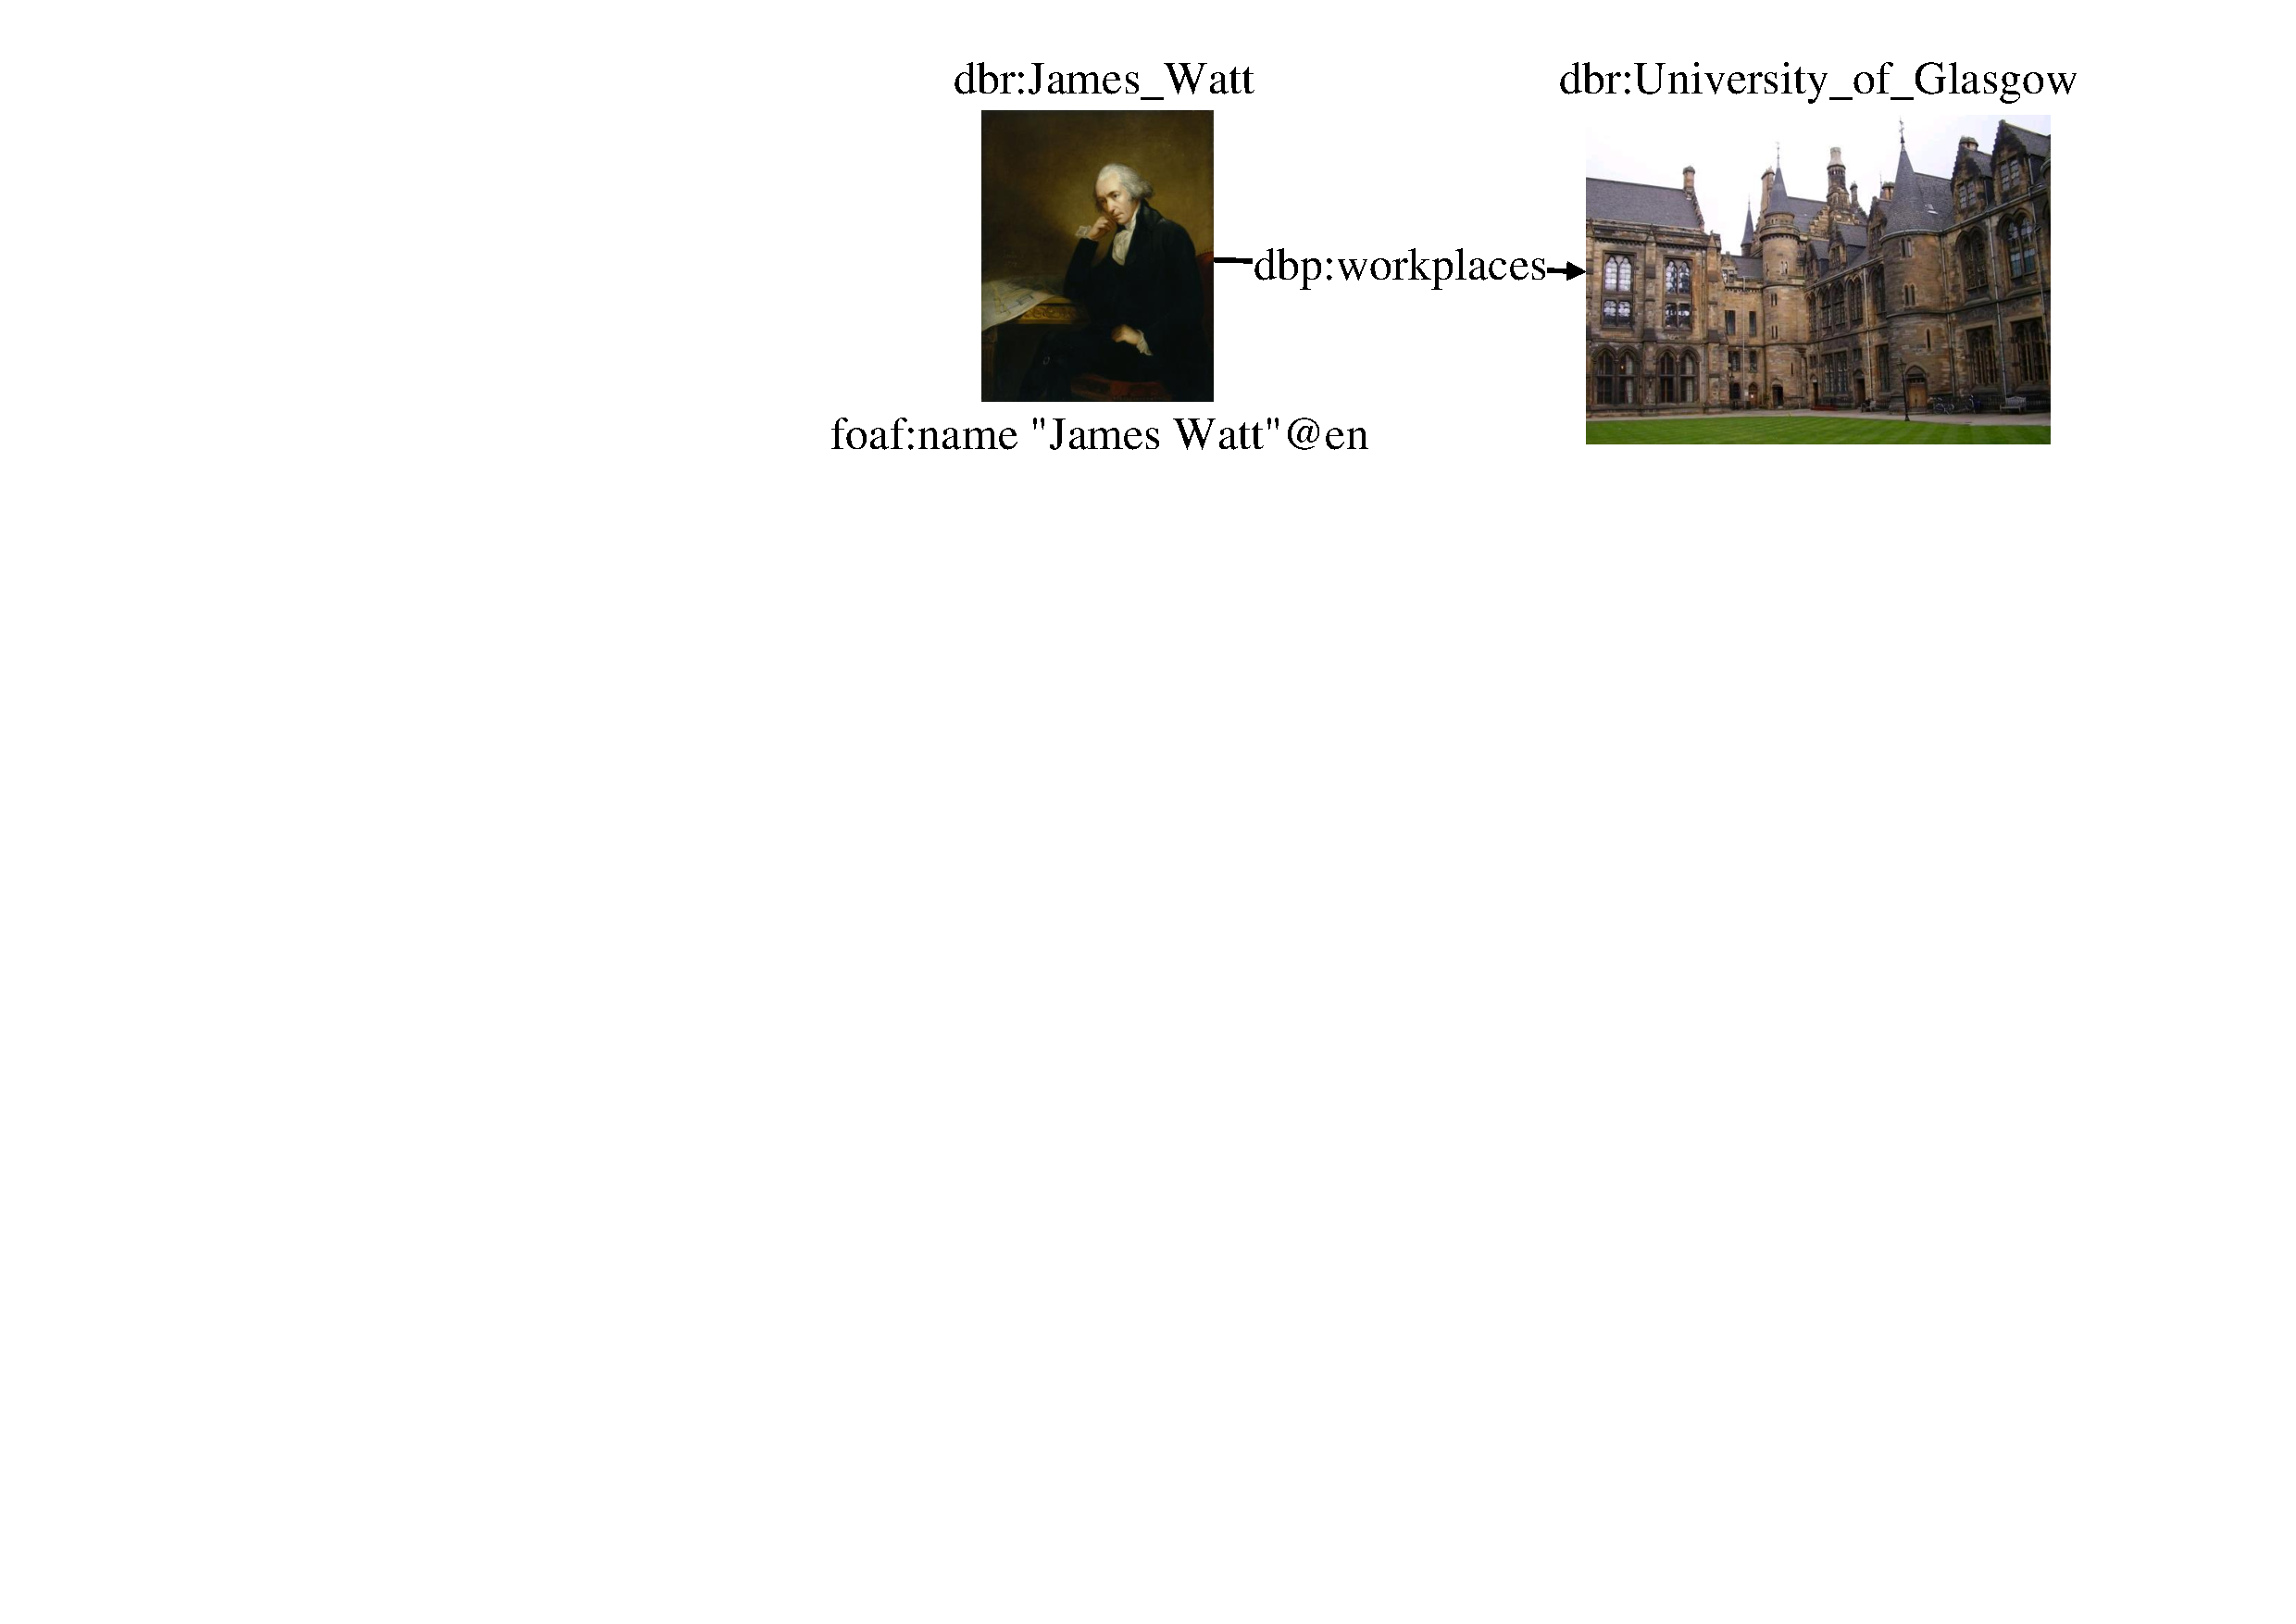
\includegraphics[width=9cm]{./figures/part1/resource.pdf}
    \caption{RDF资源}
   \label{fig:rdfresource}
\end{center}
\end{figure}

RDF的基本数据单元是一个三元组,可以表示为<主体,属性,客体>。每个三元组表示某个资源的一个属性值或者某个资源与其他资源的关系。当某条三元组描述了某个实体的属性时,其三个元素也被称为主体、属性及属性值。因此,一个知识图谱数据集可以看做一系列三元组的集合。

例如,图\ref{fig:rdftriples}中展示了一个RDF数据集的片段。这段数据截取于著名的RDF数据集DBPedia\cite{DBLP:DBpedia},描述了工业革命时期与瓦特相关的人物以及相关事物所对应的资源以及它们之间的关系。

\begin{figure}
\begin{center}
   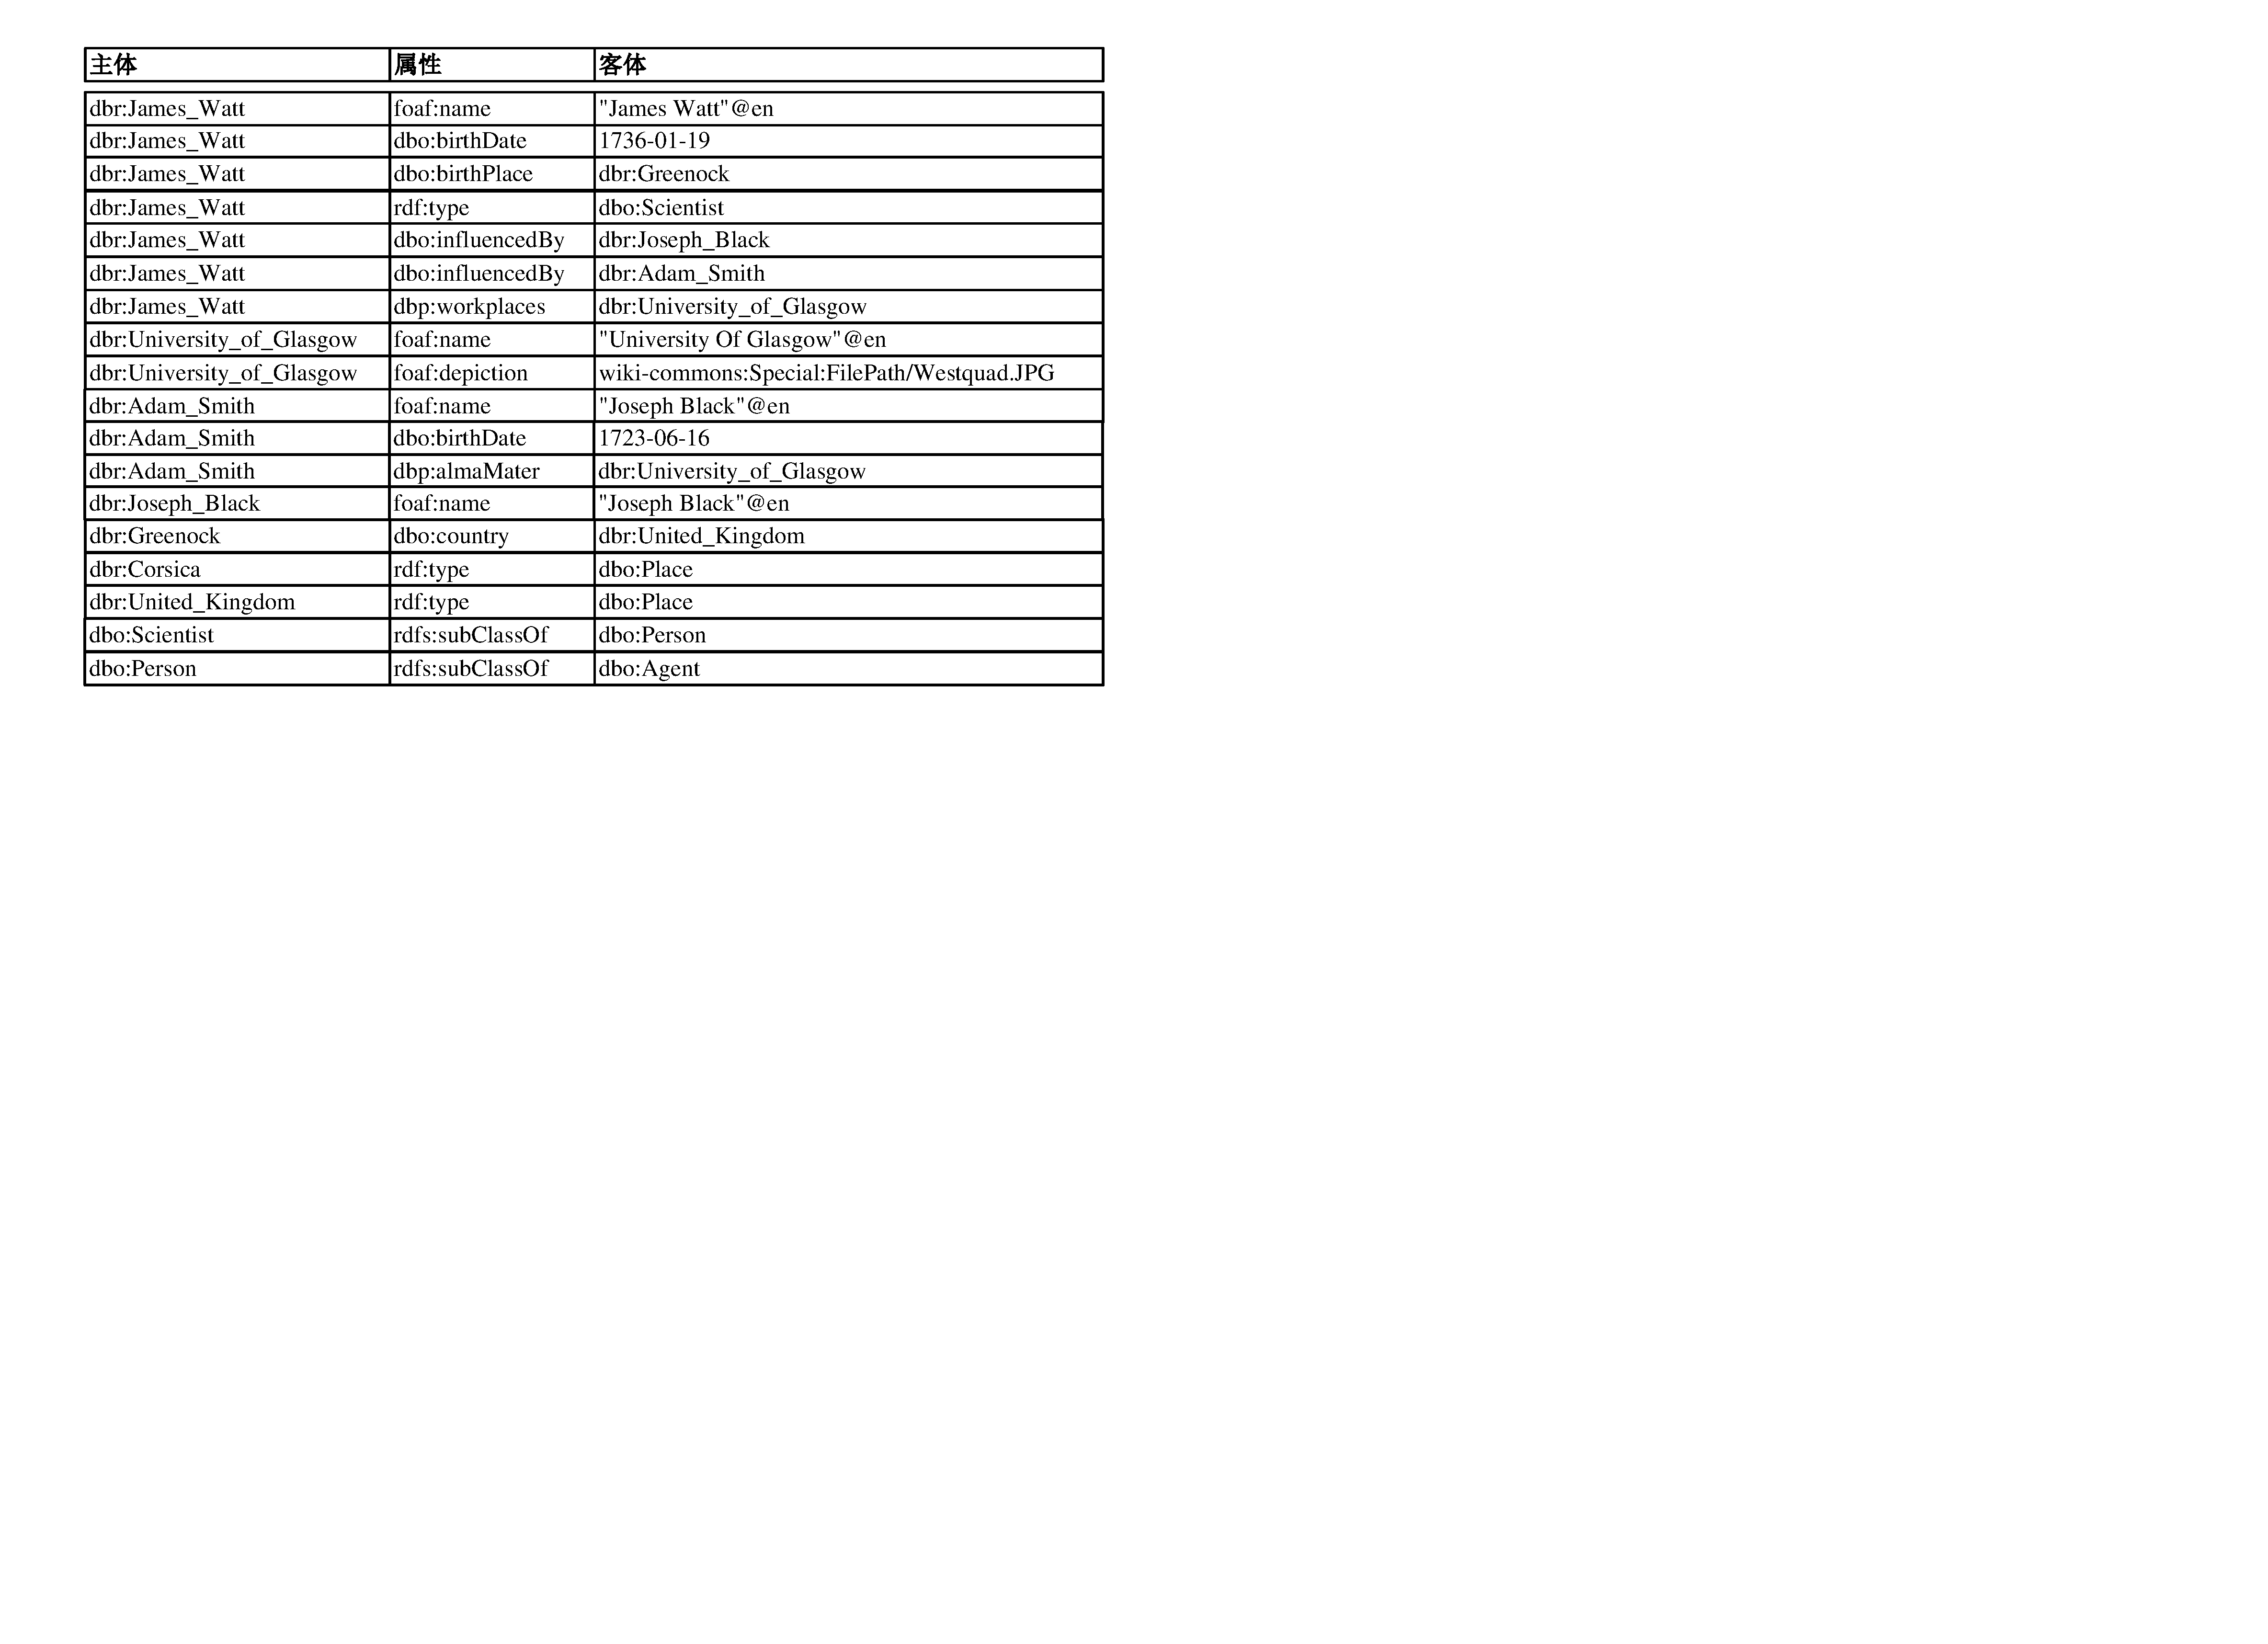
\includegraphics[width=12cm]{./figures/part1/triples.pdf}
    \caption{RDF三元组示例}
   \label{fig:rdftriples}
\end{center}
\end{figure}

%\subsection{RDF数据图模型}\label{sec:RDFGraphModel}
利用这些属性和关系,很多实体就被连接起来形成了一个大的知识图谱。按照上述的描述,我们可以发现一个知识图谱数据可以天然的被视为一个图。在这个图中,每个实体或者知识图谱数据集中出现过的字符串可以被视为图上的点,每个三元组可以视为连接主体及客体的有向边,而三元组中的谓词就可以视为有向边上的标签。相比于将知识图谱数据视为XML格式数据或三元组的集合,知识图谱的图模型包含了知识图谱数据中涵盖的语义信息。


图\ref{fig:datagraph}就是图\ref{fig:rdftriples}所示知识图谱三元组数据的图形式。如图\ref{fig:datagraph}所示,知识图谱可以表示成一个有向图,其所有的实体都是椭圆,概念是圆形,而文本点都是矩形点。


\begin{figure}
\begin{center}
   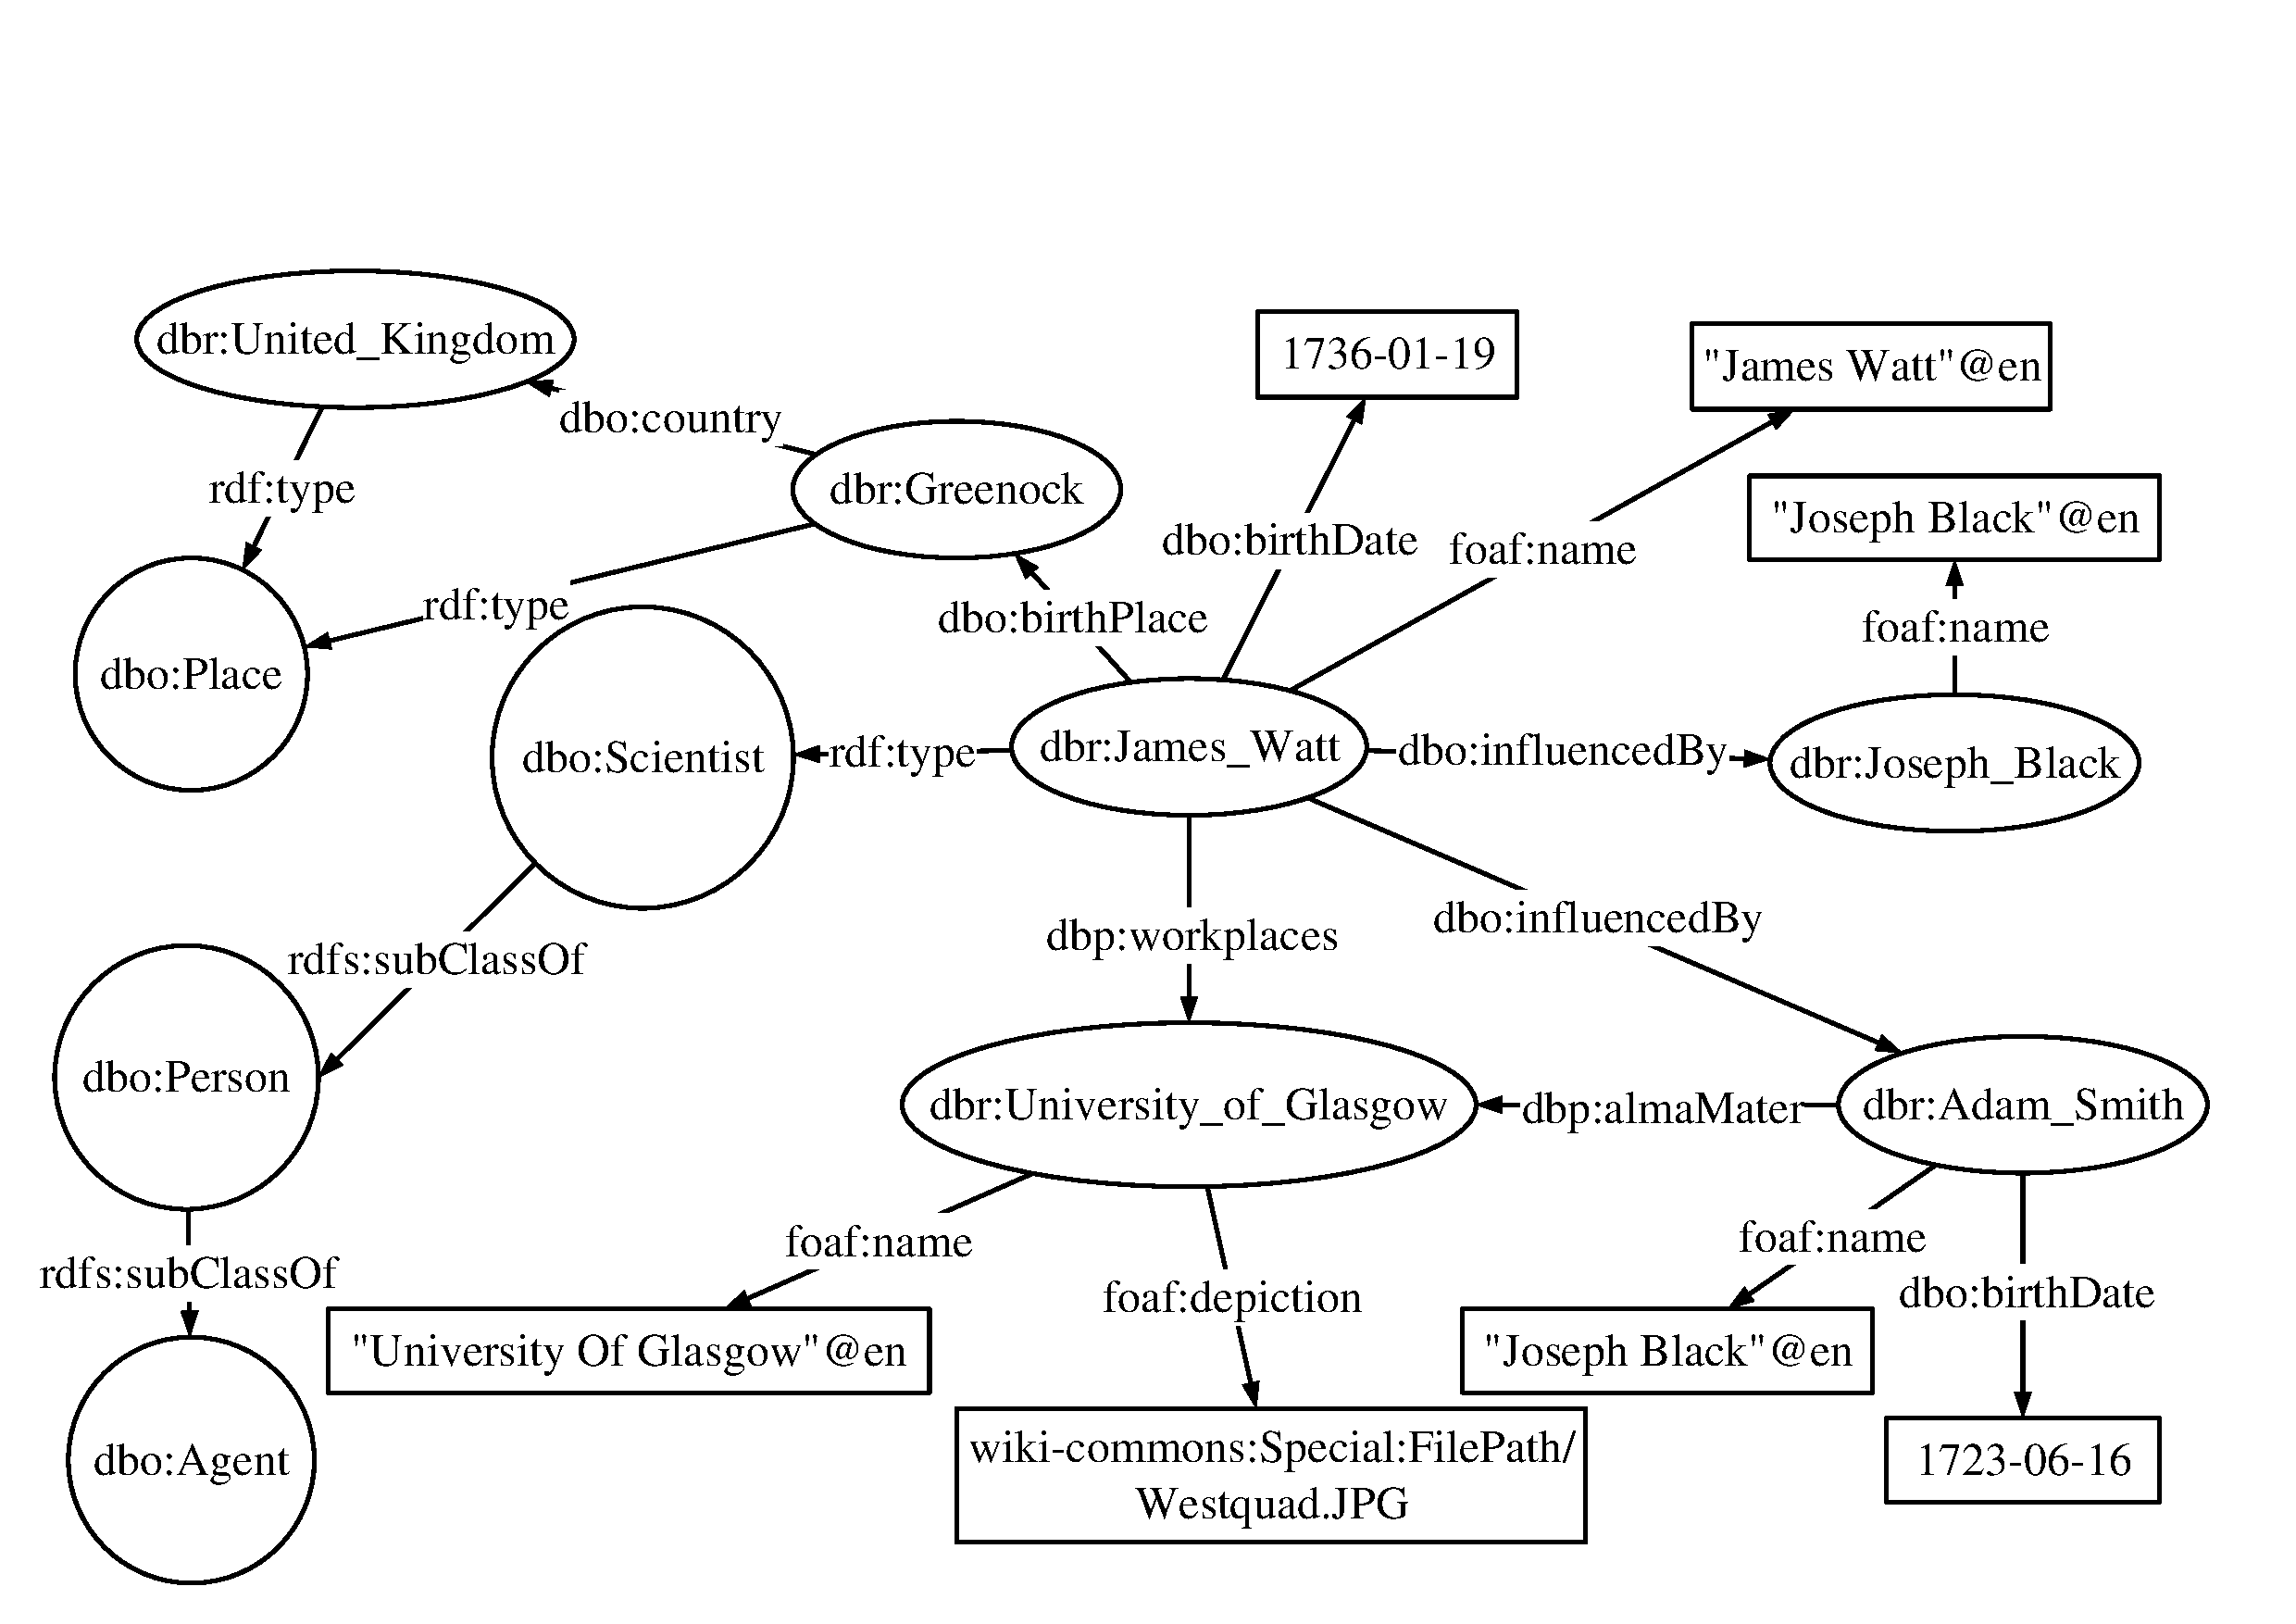
\includegraphics[width=12cm]{./figures/part1/data_graph.pdf}
    \caption{RDF数据图}
   \label{fig:datagraph}
\end{center}
\end{figure}

另一方面,SPARQL 语言与目前关系数据库中的SQL 语言是很相近的。在SPARQL 语法中,也是用SELECT 语句查询满足特定条件的RDF数据片段。具体而言,对于一个SELECT 语句中,SELECT 子句指定查询应当返回的内容,FROM 子句是指定将要使用的数据集,WHERE 子句一组三元模式组成用以指定所返回的RDF 数据片段需要满足的模式。SPARQL 语言与SQL 语言相似的这个特性方便了用户对于SPARQL 语言的使用。图\ref{fig:SPARQLStatements}(a)给出了一个针对哲学家的简单的 SPARQL 查询,目标在于查询出``在格拉斯哥大学工作的人都受到哪些人的影响?''。

\nop{
\small{
\begin{lstlisting}[language=SQL]
SELECT  ?x ?n  WHERE
{?x mainInterest Ethics.
?x influencedBy Aristotle.
?x name ?n. }
\end{lstlisting}
}
\normalsize
}

与RDF数据的图形式表示类似,一个SPARQL 查询可以表示为一个查询图\cite{VLDB2011:gStore,VLDBJ:gStore},查询中每个变量或者常量对应一个查询图上的点,每个WHERE 子句中的三元模式对应一条边。例如,图\ref{fig:SPARQLStatements}(b) 就给出了图\ref{fig:SPARQLStatements}(a)中示例SPARQL 所对应的查询图。


\begin{figure}[h]
\begin{center}
   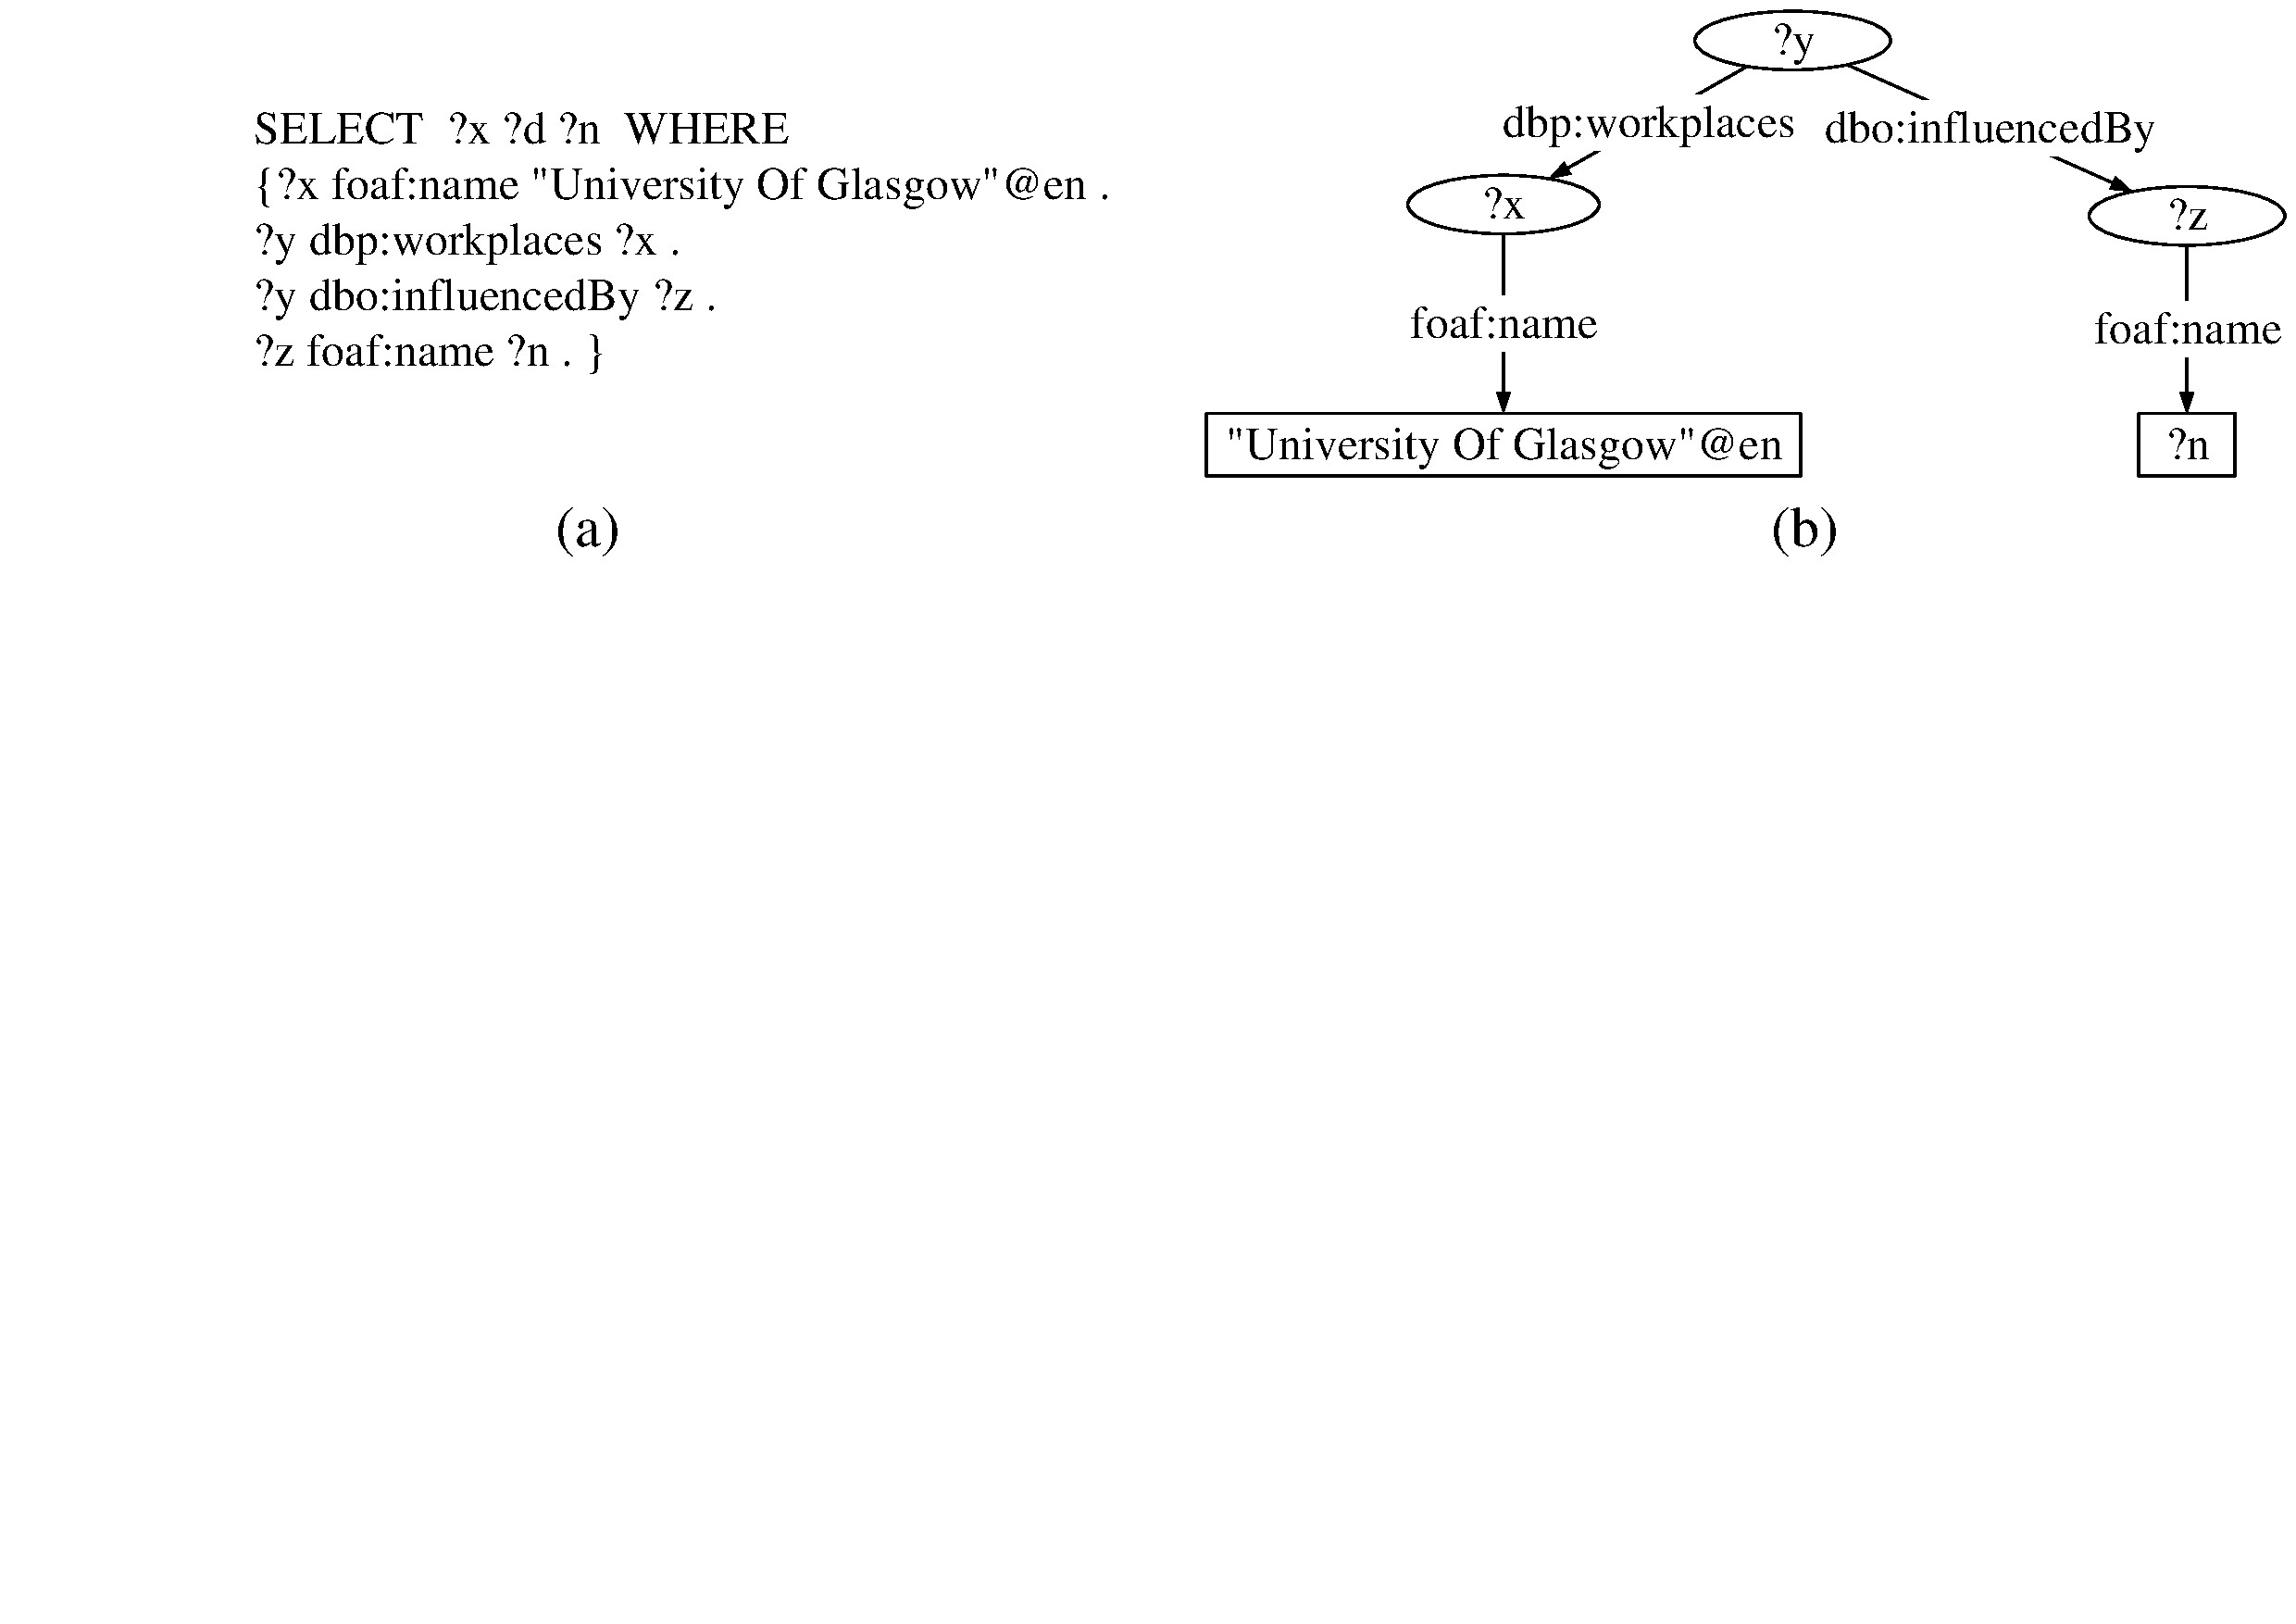
\includegraphics[width=11cm]{./figures/part1/query_graph.pdf}
    \caption{SPARQL查询图示例}
   \label{fig:SPARQLStatements}
\end{center}
\end{figure}

\section{知识图谱的价值}
知识图谱用节点和关系所组成的图谱,为真实世界的各个场景直观地建模,运用“图”这种基础性、通用性的“语言”,“高保真”地表达这个多姿多彩世界的各种关系,并且非常直观、自然、直接和高效,不需要中间过程的转换和处理——这种中间过程的转换和处理,往往把问题复杂化,或者遗漏掉很多有价值的信息。

在风控领域中,知识图谱产品为精准揭露“欺诈环”、“窝案”、“中介造假”、“洗钱”和其他复杂的欺诈手法,提供了新的方法和工具。尽管没有完美的反欺诈措施,但通过超越单个数据点并让多个节点进行联系,仍能发现一些隐藏信息,找到欺诈者的漏洞,通常这些看似正常不过的联系(关系),常常被我们忽视,但又是最有价值的反欺诈线索和风险突破口。

尽管各个风险场景的业务风险不同,其欺诈方式也不同,但都有一个非常重要的共同点——欺诈依赖于信息不对称和间接层,且它们可以通过知识图谱的关联分析被揭示出来,高级欺诈也难以“隐身”。

凡是有关系的地方都可以用到知识图谱,事实上,知识图谱已经成功俘获了大量客户,且客户数量和应用领域还在不断增长中,包括沃尔玛、领英、阿迪达斯、惠普、FT金融时报等知名企业和机构。

目前知识图谱产品的客户行业,分类主要集中在:社交网络、人力资源与招聘、金融、保险、零售、广告、物流、通信、IT、制造业、传媒、医疗、电子商务和物流等领域。在风控领域中,知识图谱类产品主要应用于反欺诈、反洗钱、互联网授信、保险欺诈、银行欺诈、电商欺诈、项目审计作假、企业关系分析、罪犯追踪等场景中。

那相比传统数据存储和计算方式,知识图谱的优势显现在哪里呢?

\begin{itemize}
  \item \textbf{关系的表达能力强.}传统数据库通常通过表格、字段等方式进行读取,而关系的层级及表达方式多种多样,且基于图论和概率图模型,可以处理复杂多样的关联分析,满足企业各种角色关系的分析和管理需要。
  \item \textbf{像人类思考一样去做分析.}基于知识图谱的交互探索式分析,可以模拟人的思考过程去发现、求证、推理,业务人员自己就可以完成全部过程,不需要专业人员的协助。
  \item \textbf{知识学习.}利用交互式机器学习技术,支持根据推理、纠错、标注等交互动作的学习功能,不断沉淀知识逻辑和模型,提高系统智能性,将知识沉淀在企业内部,降低对经验的依赖。
  \item \textbf{高速反馈.}图式的数据存储方式,相比传统存储方式,数据调取速度更快,图库可计算超过百万潜在的实体的属性分布,可实现秒级返回结果,真正实现人机互动的实时响应,让用户可以做到即时决策。
\end{itemize}



\section{知识图谱的应用}
知识图谱的应用场景很多,在不同行业不同领域也有广泛应用。在本书中,我们将以几个目前比较常见的应用场景为例像大家介绍一下知识图谱应用。

\subsection{基于金融知识图谱的股权分析}

\subsection{基于医疗知识图谱的辅助诊断}


\subsection{基于知识图谱的智能问答}